\documentclass[1p]{elsarticle_modified}
%\bibliographystyle{elsarticle-num}

%\usepackage[colorlinks]{hyperref}
%\usepackage{abbrmath_seonhwa} %\Abb, \Ascr, \Acal ,\Abf, \Afrak
\usepackage{amsfonts}
\usepackage{amssymb}
\usepackage{amsmath}
\usepackage{amsthm}
\usepackage{scalefnt}
\usepackage{amsbsy}
\usepackage{kotex}
\usepackage{caption}
\usepackage{subfig}
\usepackage{color}
\usepackage{graphicx}
\usepackage{xcolor} %% white, black, red, green, blue, cyan, magenta, yellow
\usepackage{float}
\usepackage{setspace}
\usepackage{hyperref}

\usepackage{tikz}
\usetikzlibrary{arrows}

\usepackage{multirow}
\usepackage{array} % fixed length table
\usepackage{hhline}

%%%%%%%%%%%%%%%%%%%%%
\makeatletter
\renewcommand*\env@matrix[1][\arraystretch]{%
	\edef\arraystretch{#1}%
	\hskip -\arraycolsep
	\let\@ifnextchar\new@ifnextchar
	\array{*\c@MaxMatrixCols c}}
\makeatother %https://tex.stackexchange.com/questions/14071/how-can-i-increase-the-line-spacing-in-a-matrix
%%%%%%%%%%%%%%%

\usepackage[normalem]{ulem}

\newcommand{\msout}[1]{\ifmmode\text{\sout{\ensuremath{#1}}}\else\sout{#1}\fi}
%SOURCE: \msout is \stkout macro in https://tex.stackexchange.com/questions/20609/strikeout-in-math-mode

\newcommand{\cancel}[1]{
	\ifmmode
	{\color{red}\msout{#1}}
	\else
	{\color{red}\sout{#1}}
	\fi
}

\newcommand{\add}[1]{
	{\color{blue}\uwave{#1}}
}

\newcommand{\replace}[2]{
	\ifmmode
	{\color{red}\msout{#1}}{\color{blue}\uwave{#2}}
	\else
	{\color{red}\sout{#1}}{\color{blue}\uwave{#2}}
	\fi
}

\newcommand{\Sol}{\mathcal{S}} %segment
\newcommand{\D}{D} %diagram
\newcommand{\A}{\mathcal{A}} %arc


%%%%%%%%%%%%%%%%%%%%%%%%%%%%%5 test

\def\sl{\operatorname{\textup{SL}}(2,\Cbb)}
\def\psl{\operatorname{\textup{PSL}}(2,\Cbb)}
\def\quan{\mkern 1mu \triangleright \mkern 1mu}

\theoremstyle{definition}
\newtheorem{thm}{Theorem}[section]
\newtheorem{prop}[thm]{Proposition}
\newtheorem{lem}[thm]{Lemma}
\newtheorem{ques}[thm]{Question}
\newtheorem{cor}[thm]{Corollary}
\newtheorem{defn}[thm]{Definition}
\newtheorem{exam}[thm]{Example}
\newtheorem{rmk}[thm]{Remark}
\newtheorem{alg}[thm]{Algorithm}

\newcommand{\I}{\sqrt{-1}}
\begin{document}

%\begin{frontmatter}
%
%\title{Boundary parabolic representations of knots up to 8 crossings}
%
%%% Group authors per affiliation:
%\author{Yunhi Cho} 
%\address{Department of Mathematics, University of Seoul, Seoul, Korea}
%\ead{yhcho@uos.ac.kr}
%
%
%\author{Seonhwa Kim} %\fnref{s_kim}}
%\address{Center for Geometry and Physics, Institute for Basic Science, Pohang, 37673, Korea}
%\ead{ryeona17@ibs.re.kr}
%
%\author{Hyuk Kim}
%\address{Department of Mathematical Sciences, Seoul National University, Seoul 08826, Korea}
%\ead{hyukkim@snu.ac.kr}
%
%\author{Seokbeom Yoon}
%\address{Department of Mathematical Sciences, Seoul National University, Seoul, 08826,  Korea}
%\ead{sbyoon15@snu.ac.kr}
%
%\begin{abstract}
%We find all boundary parabolic representation of knots up to 8 crossings.
%
%\end{abstract}
%\begin{keyword}
%    \MSC[2010] 57M25 
%\end{keyword}
%
%\end{frontmatter}

%\linenumbers
%\tableofcontents
%
\newcommand\colored[1]{\textcolor{white}{\rule[-0.35ex]{0.8em}{1.4ex}}\kern-0.8em\color{red} #1}%
%\newcommand\colored[1]{\textcolor{white}{ #1}\kern-2.17ex	\textcolor{white}{ #1}\kern-1.81ex	\textcolor{white}{ #1}\kern-2.15ex\color{red}#1	}

{\Large $\underline{12a_{1280}~(K12a_{1280})}$}

\setlength{\tabcolsep}{10pt}
\renewcommand{\arraystretch}{1.6}
\vspace{1cm}\begin{tabular}{m{100pt}>{\centering\arraybackslash}m{274pt}}
\multirow{5}{120pt}{
	\centering
	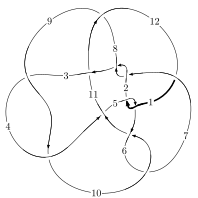
\includegraphics[width=112pt]{../../../GIT/diagram.site/Diagrams/png/2081_12a_1280.png}\\
\ \ \ A knot diagram\footnotemark}&
\allowdisplaybreaks
\textbf{Linearized knot diagam} \\
\cline{2-2}
 &
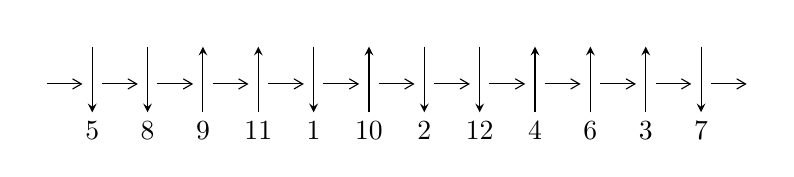
\begin{tikzpicture}[x=20pt, y=17pt]
	% nodes
	\node (C0) at (0, 0) {};
	\node (C1) at (1, 0) {};
	\node (C1U) at (1, +1) {};
	\node (C1D) at (1, -1) {5};

	\node (C2) at (2, 0) {};
	\node (C2U) at (2, +1) {};
	\node (C2D) at (2, -1) {8};

	\node (C3) at (3, 0) {};
	\node (C3U) at (3, +1) {};
	\node (C3D) at (3, -1) {9};

	\node (C4) at (4, 0) {};
	\node (C4U) at (4, +1) {};
	\node (C4D) at (4, -1) {11};

	\node (C5) at (5, 0) {};
	\node (C5U) at (5, +1) {};
	\node (C5D) at (5, -1) {1};

	\node (C6) at (6, 0) {};
	\node (C6U) at (6, +1) {};
	\node (C6D) at (6, -1) {10};

	\node (C7) at (7, 0) {};
	\node (C7U) at (7, +1) {};
	\node (C7D) at (7, -1) {2};

	\node (C8) at (8, 0) {};
	\node (C8U) at (8, +1) {};
	\node (C8D) at (8, -1) {12};

	\node (C9) at (9, 0) {};
	\node (C9U) at (9, +1) {};
	\node (C9D) at (9, -1) {4};

	\node (C10) at (10, 0) {};
	\node (C10U) at (10, +1) {};
	\node (C10D) at (10, -1) {6};

	\node (C11) at (11, 0) {};
	\node (C11U) at (11, +1) {};
	\node (C11D) at (11, -1) {3};

	\node (C12) at (12, 0) {};
	\node (C12U) at (12, +1) {};
	\node (C12D) at (12, -1) {7};
	\node (C13) at (13, 0) {};

	% arrows
	\draw[->,>={angle 60}]
	(C0) edge (C1) (C1) edge (C2) (C2) edge (C3) (C3) edge (C4) (C4) edge (C5) (C5) edge (C6) (C6) edge (C7) (C7) edge (C8) (C8) edge (C9) (C9) edge (C10) (C10) edge (C11) (C11) edge (C12) (C12) edge (C13) ;	\draw[->,>=stealth]
	(C1U) edge (C1D) (C2U) edge (C2D) (C3D) edge (C3U) (C4D) edge (C4U) (C5U) edge (C5D) (C6D) edge (C6U) (C7U) edge (C7D) (C8U) edge (C8D) (C9D) edge (C9U) (C10D) edge (C10U) (C11D) edge (C11U) (C12U) edge (C12D) ;
	\end{tikzpicture} \\
\hhline{~~} \\& 
\textbf{Solving Sequence} \\ \cline{2-2} 
 &
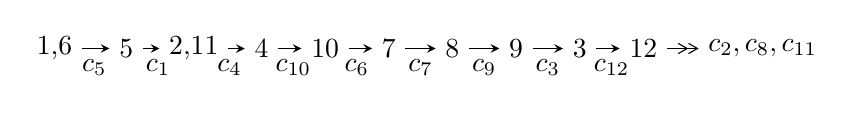
\begin{tikzpicture}[x=23pt, y=7pt]
	% node
	\node (A0) at (-1/8, 0) {1,6};
	\node (A1) at (1, 0) {5};
	\node (A2) at (33/16, 0) {2,11};
	\node (A3) at (25/8, 0) {4};
	\node (A4) at (33/8, 0) {10};
	\node (A5) at (41/8, 0) {7};
	\node (A6) at (49/8, 0) {8};
	\node (A7) at (57/8, 0) {9};
	\node (A8) at (65/8, 0) {3};
	\node (A9) at (73/8, 0) {12};
	\node (C1) at (1/2, -1) {$c_{5}$};
	\node (C2) at (3/2, -1) {$c_{1}$};
	\node (C3) at (21/8, -1) {$c_{4}$};
	\node (C4) at (29/8, -1) {$c_{10}$};
	\node (C5) at (37/8, -1) {$c_{6}$};
	\node (C6) at (45/8, -1) {$c_{7}$};
	\node (C7) at (53/8, -1) {$c_{9}$};
	\node (C8) at (61/8, -1) {$c_{3}$};
	\node (C9) at (69/8, -1) {$c_{12}$};
	\node (A10) at (11, 0) {$c_{2},c_{8},c_{11}$};

	% edge
	\draw[->,>=stealth]	
	(A0) edge (A1) (A1) edge (A2) (A2) edge (A3) (A3) edge (A4) (A4) edge (A5) (A5) edge (A6) (A6) edge (A7) (A7) edge (A8) (A8) edge (A9) ;
	\draw[->>,>={angle 60}]	
	(A9) edge (A10);
\end{tikzpicture} \\ 

\end{tabular} \\

\footnotetext{
The image of knot diagram is generated by the software ``\textbf{Draw programme}" developed by Andrew Bartholomew(\url{http://www.layer8.co.uk/maths/draw/index.htm\#Running-draw}), where we modified some parts for our purpose(\url{https://github.com/CATsTAILs/LinksPainter}).
}\phantom \\ \newline 
\centering \textbf{Ideals for irreducible components\footnotemark of $X_{\text{par}}$} 
 
\begin{align*}
I^u_{1}&=\langle 
-1.89817\times10^{771} u^{159}-8.88168\times10^{771} u^{158}+\cdots+1.85109\times10^{773} b+7.26797\times10^{773},\\
\phantom{I^u_{1}}&\phantom{= \langle  }-7.79658\times10^{780} u^{159}+8.42830\times10^{780} u^{158}+\cdots+1.47412\times10^{783} a+4.88030\times10^{784},\\
\phantom{I^u_{1}}&\phantom{= \langle  }u^{160}+5 u^{159}+\cdots+1034 u+763\rangle \\
I^u_{2}&=\langle 
-1.11952\times10^{18} u^{39}+9.08577\times10^{17} u^{38}+\cdots+4.95466\times10^{16} b+1.44944\times10^{18},\\
\phantom{I^u_{2}}&\phantom{= \langle  }2.55914\times10^{20} u^{39}-1.19489\times10^{22} u^{38}+\cdots+3.04167\times10^{20} a-5.39997\times10^{22},\;u^{40}+10 u^{38}+\cdots-2 u+1\rangle \\
\\
\end{align*}
\raggedright * 2 irreducible components of $\dim_{\mathbb{C}}=0$, with total 200 representations.\\
\footnotetext{All coefficients of polynomials are rational numbers. But the coefficients are sometimes approximated in decimal forms when there is not enough margin.}
\newpage
\renewcommand{\arraystretch}{1}
\centering \section*{I. $I^u_{1}= \langle -1.90\times10^{771} u^{159}-8.88\times10^{771} u^{158}+\cdots+1.85\times10^{773} b+7.27\times10^{773},\;-7.80\times10^{780} u^{159}+8.43\times10^{780} u^{158}+\cdots+1.47\times10^{783} a+4.88\times10^{784},\;u^{160}+5 u^{159}+\cdots+1034 u+763 \rangle$}
\flushleft \textbf{(i) Arc colorings}\\
\begin{tabular}{m{7pt} m{180pt} m{7pt} m{180pt} }
\flushright $a_{1}=$&$\begin{pmatrix}0\\u\end{pmatrix}$ \\
\flushright $a_{6}=$&$\begin{pmatrix}1\\0\end{pmatrix}$ \\
\flushright $a_{5}=$&$\begin{pmatrix}1\\- u^2\end{pmatrix}$ \\
\flushright $a_{2}=$&$\begin{pmatrix}- u\\u^3+u\end{pmatrix}$ \\
\flushright $a_{11}=$&$\begin{pmatrix}0.00528898 u^{159}-0.00571753 u^{158}+\cdots-31.2417 u-33.1066\\0.0102543 u^{159}+0.0479809 u^{158}+\cdots-1.97258 u-3.92632\end{pmatrix}$ \\
\flushright $a_{4}=$&$\begin{pmatrix}0.00208837 u^{159}+0.0175818 u^{158}+\cdots+93.9097 u+25.1074\\-0.00146282 u^{159}-0.00856543 u^{158}+\cdots-6.96135 u-0.610702\end{pmatrix}$ \\
\flushright $a_{10}=$&$\begin{pmatrix}-0.00496536 u^{159}-0.0536984 u^{158}+\cdots-29.2691 u-29.1803\\0.0102543 u^{159}+0.0479809 u^{158}+\cdots-1.97258 u-3.92632\end{pmatrix}$ \\
\flushright $a_{7}=$&$\begin{pmatrix}-0.00321433 u^{159}-0.00722482 u^{158}+\cdots-20.2256 u+8.49310\\0.0134674 u^{159}+0.0671173 u^{158}+\cdots+23.7049 u+7.19324\end{pmatrix}$ \\
\flushright $a_{8}=$&$\begin{pmatrix}0.00196200 u^{159}+0.0180792 u^{158}+\cdots-8.19279 u+12.9535\\0.0119696 u^{159}+0.0581319 u^{158}+\cdots+15.0244 u+2.29208\end{pmatrix}$ \\
\flushright $a_{9}=$&$\begin{pmatrix}0.0495996 u^{159}+0.266425 u^{158}+\cdots+129.695 u+41.9874\\-0.00966189 u^{159}-0.0379134 u^{158}+\cdots-8.27916 u+7.42179\end{pmatrix}$ \\
\flushright $a_{3}=$&$\begin{pmatrix}-0.000282697 u^{159}-0.00229252 u^{158}+\cdots+4.31477 u+9.56055\\0.00667690 u^{159}+0.0315444 u^{158}+\cdots+12.8545 u-0.248031\end{pmatrix}$ \\
\flushright $a_{12}=$&$\begin{pmatrix}0.00641506 u^{159}+0.0525232 u^{158}+\cdots+20.9392 u+4.33778\\0.000688568 u^{159}+0.00147807 u^{158}+\cdots+5.68861 u+3.15312\end{pmatrix}$\\&\end{tabular}
\flushleft \textbf{(ii) Obstruction class $= -1$}\\~\\
\flushleft \textbf{(iii) Cusp Shapes $= 0.0110703 u^{159}+0.0900993 u^{158}+\cdots-86.6660 u+30.0672$}\\~\\
\newpage\renewcommand{\arraystretch}{1}
\flushleft \textbf{(iv) u-Polynomials at the component}\newline \\
\begin{tabular}{m{50pt}|m{274pt}}
Crossings & \hspace{64pt}u-Polynomials at each crossing \\
\hline $$\begin{aligned}c_{1},c_{5}\end{aligned}$$&$\begin{aligned}
&u^{160}+5 u^{159}+\cdots+1034 u+763
\end{aligned}$\\
\hline $$\begin{aligned}c_{2},c_{7}\end{aligned}$$&$\begin{aligned}
&u^{160}+u^{159}+\cdots+79965 u+7417
\end{aligned}$\\
\hline $$\begin{aligned}c_{3},c_{9}\end{aligned}$$&$\begin{aligned}
&u^{160}- u^{159}+\cdots-79965 u+7417
\end{aligned}$\\
\hline $$\begin{aligned}c_{4}\end{aligned}$$&$\begin{aligned}
&u^{160}+u^{159}+\cdots+6487992 u+714773
\end{aligned}$\\
\hline $$\begin{aligned}c_{6},c_{10}\end{aligned}$$&$\begin{aligned}
&u^{160}-5 u^{159}+\cdots-1034 u+763
\end{aligned}$\\
\hline $$\begin{aligned}c_{8}\end{aligned}$$&$\begin{aligned}
&u^{160}+7 u^{159}+\cdots+60 u+7
\end{aligned}$\\
\hline $$\begin{aligned}c_{11}\end{aligned}$$&$\begin{aligned}
&u^{160}-7 u^{159}+\cdots-60 u+7
\end{aligned}$\\
\hline $$\begin{aligned}c_{12}\end{aligned}$$&$\begin{aligned}
&u^{160}- u^{159}+\cdots-6487992 u+714773
\end{aligned}$\\
\hline
\end{tabular}\\~\\
\newpage\renewcommand{\arraystretch}{1}
\flushleft \textbf{(v) Riley Polynomials at the component}\newline \\
\begin{tabular}{m{50pt}|m{274pt}}
Crossings & \hspace{64pt}Riley Polynomials at each crossing \\
\hline $$\begin{aligned}c_{1},c_{5},c_{6}\\c_{10}\end{aligned}$$&$\begin{aligned}
&y^{160}+81 y^{159}+\cdots+13136378 y+582169
\end{aligned}$\\
\hline $$\begin{aligned}c_{2},c_{3},c_{7}\\c_{9}\end{aligned}$$&$\begin{aligned}
&y^{160}-115 y^{159}+\cdots+324258557 y+55011889
\end{aligned}$\\
\hline $$\begin{aligned}c_{4},c_{12}\end{aligned}$$&$\begin{aligned}
&y^{160}-7 y^{159}+\cdots+4855248205898 y+510900441529
\end{aligned}$\\
\hline $$\begin{aligned}c_{8},c_{11}\end{aligned}$$&$\begin{aligned}
&y^{160}+7 y^{159}+\cdots+1832 y+49
\end{aligned}$\\
\hline
\end{tabular}\\~\\
\newpage\flushleft \textbf{(vi) Complex Volumes and Cusp Shapes}
$$\begin{array}{c|c|c}  
\text{Solutions to }I^u_{1}& \I (\text{vol} + \sqrt{-1}CS) & \text{Cusp shape}\\
 \hline 
\begin{aligned}
u &= -0.385490 + 0.927127 I \\
a &= \phantom{-}1.27250 - 1.33805 I \\
b &= \phantom{-}1.30399 - 0.73093 I\end{aligned}
 & \phantom{-}4.40812 - 1.23041 I & \phantom{-0.000000 } 0 \\ \hline\begin{aligned}
u &= -0.385490 - 0.927127 I \\
a &= \phantom{-}1.27250 + 1.33805 I \\
b &= \phantom{-}1.30399 + 0.73093 I\end{aligned}
 & \phantom{-}4.40812 + 1.23041 I & \phantom{-0.000000 } 0 \\ \hline\begin{aligned}
u &= -0.294481 + 0.965440 I \\
a &= \phantom{-}2.94395 + 0.99740 I \\
b &= \phantom{-}0.356688 + 1.203140 I\end{aligned}
 & -2.58230 + 7.66961 I & \phantom{-0.000000 } 0 \\ \hline\begin{aligned}
u &= -0.294481 - 0.965440 I \\
a &= \phantom{-}2.94395 - 0.99740 I \\
b &= \phantom{-}0.356688 - 1.203140 I\end{aligned}
 & -2.58230 - 7.66961 I & \phantom{-0.000000 } 0 \\ \hline\begin{aligned}
u &= \phantom{-}0.457188 + 0.877846 I \\
a &= \phantom{-}2.09641 - 0.62542 I \\
b &= \phantom{-}0.530075 - 1.123270 I\end{aligned}
 & -6.63354 - 0.43992 I & \phantom{-0.000000 } 0 \\ \hline\begin{aligned}
u &= \phantom{-}0.457188 - 0.877846 I \\
a &= \phantom{-}2.09641 + 0.62542 I \\
b &= \phantom{-}0.530075 + 1.123270 I\end{aligned}
 & -6.63354 + 0.43992 I & \phantom{-0.000000 } 0 \\ \hline\begin{aligned}
u &= -0.193630 + 0.965913 I \\
a &= -1.71135 + 0.57654 I \\
b &= -1.203960 + 0.670041 I\end{aligned}
 & \phantom{-}3.46403 - 0.49869 I & \phantom{-0.000000 } 0 \\ \hline\begin{aligned}
u &= -0.193630 - 0.965913 I \\
a &= -1.71135 - 0.57654 I \\
b &= -1.203960 - 0.670041 I\end{aligned}
 & \phantom{-}3.46403 + 0.49869 I & \phantom{-0.000000 } 0 \\ \hline\begin{aligned}
u &= -0.630257 + 0.821670 I \\
a &= \phantom{-}1.18016 - 1.23585 I \\
b &= \phantom{-}0.842114 + 0.831002 I\end{aligned}
 & \phantom{-}3.14638 + 5.48393 I & \phantom{-0.000000 } 0 \\ \hline\begin{aligned}
u &= -0.630257 - 0.821670 I \\
a &= \phantom{-}1.18016 + 1.23585 I \\
b &= \phantom{-}0.842114 - 0.831002 I\end{aligned}
 & \phantom{-}3.14638 - 5.48393 I & \phantom{-0.000000 } 0\\
 \hline 
 \end{array}$$\newpage$$\begin{array}{c|c|c}  
\text{Solutions to }I^u_{1}& \I (\text{vol} + \sqrt{-1}CS) & \text{Cusp shape}\\
 \hline 
\begin{aligned}
u &= -0.528497 + 0.902931 I \\
a &= \phantom{-}0.459469 + 0.183830 I \\
b &= -0.06658 + 1.53283 I\end{aligned}
 & -4.48952 + 8.79836 I & \phantom{-0.000000 } 0 \\ \hline\begin{aligned}
u &= -0.528497 - 0.902931 I \\
a &= \phantom{-}0.459469 - 0.183830 I \\
b &= -0.06658 - 1.53283 I\end{aligned}
 & -4.48952 - 8.79836 I & \phantom{-0.000000 } 0 \\ \hline\begin{aligned}
u &= \phantom{-}0.423235 + 0.960586 I \\
a &= -2.26309 + 0.72628 I \\
b &= -0.200193 + 1.041780 I\end{aligned}
 & -6.16928 - 4.22992 I & \phantom{-0.000000 } 0 \\ \hline\begin{aligned}
u &= \phantom{-}0.423235 - 0.960586 I \\
a &= -2.26309 - 0.72628 I \\
b &= -0.200193 - 1.041780 I\end{aligned}
 & -6.16928 + 4.22992 I & \phantom{-0.000000 } 0 \\ \hline\begin{aligned}
u &= \phantom{-}1.042900 + 0.163804 I \\
a &= \phantom{-}0.156926 - 0.138138 I \\
b &= \phantom{-}0.513923 + 1.144070 I\end{aligned}
 & \phantom{-}1.55339 + 8.26333 I & \phantom{-0.000000 } 0 \\ \hline\begin{aligned}
u &= \phantom{-}1.042900 - 0.163804 I \\
a &= \phantom{-}0.156926 + 0.138138 I \\
b &= \phantom{-}0.513923 - 1.144070 I\end{aligned}
 & \phantom{-}1.55339 - 8.26333 I & \phantom{-0.000000 } 0 \\ \hline\begin{aligned}
u &= -1.059430 + 0.037653 I \\
a &= \phantom{-}0.141751 - 0.253958 I \\
b &= -0.189671 + 1.071480 I\end{aligned}
 & -3.62698 - 1.64070 I & \phantom{-0.000000 } 0 \\ \hline\begin{aligned}
u &= -1.059430 - 0.037653 I \\
a &= \phantom{-}0.141751 + 0.253958 I \\
b &= -0.189671 - 1.071480 I\end{aligned}
 & -3.62698 + 1.64070 I & \phantom{-0.000000 } 0 \\ \hline\begin{aligned}
u &= \phantom{-}0.339681 + 1.004880 I \\
a &= \phantom{-}1.171080 - 0.163992 I \\
b &= \phantom{-}0.339681 - 1.004880 I\end{aligned}
 & \phantom{-0.000000 -}0.481977 I & \phantom{-0.000000 } 0 \\ \hline\begin{aligned}
u &= \phantom{-}0.339681 - 1.004880 I \\
a &= \phantom{-}1.171080 + 0.163992 I \\
b &= \phantom{-}0.339681 + 1.004880 I\end{aligned}
 & \phantom{-0.000000 } -0.481977 I & \phantom{-0.000000 } 0\\
 \hline 
 \end{array}$$\newpage$$\begin{array}{c|c|c}  
\text{Solutions to }I^u_{1}& \I (\text{vol} + \sqrt{-1}CS) & \text{Cusp shape}\\
 \hline 
\begin{aligned}
u &= -0.200193 + 1.041780 I \\
a &= \phantom{-}1.85659 - 0.90395 I \\
b &= \phantom{-}0.423235 + 0.960586 I\end{aligned}
 & \phantom{-}6.16928 + 4.22992 I & \phantom{-0.000000 } 0 \\ \hline\begin{aligned}
u &= -0.200193 - 1.041780 I \\
a &= \phantom{-}1.85659 + 0.90395 I \\
b &= \phantom{-}0.423235 - 0.960586 I\end{aligned}
 & \phantom{-}6.16928 - 4.22992 I & \phantom{-0.000000 } 0 \\ \hline\begin{aligned}
u &= \phantom{-}0.409874 + 0.982147 I \\
a &= -1.51896 - 0.85860 I \\
b &= -0.646848 + 0.242634 I\end{aligned}
 & \phantom{-}4.95212 - 3.37858 I & \phantom{-0.000000 } 0 \\ \hline\begin{aligned}
u &= \phantom{-}0.409874 - 0.982147 I \\
a &= -1.51896 + 0.85860 I \\
b &= -0.646848 - 0.242634 I\end{aligned}
 & \phantom{-}4.95212 + 3.37858 I & \phantom{-0.000000 } 0 \\ \hline\begin{aligned}
u &= \phantom{-}0.441987 + 0.988216 I \\
a &= -1.64389 - 0.14711 I \\
b &= -0.590734 + 1.176550 I\end{aligned}
 & \phantom{-}0.59941 - 4.40862 I & \phantom{-0.000000 } 0 \\ \hline\begin{aligned}
u &= \phantom{-}0.441987 - 0.988216 I \\
a &= -1.64389 + 0.14711 I \\
b &= -0.590734 - 1.176550 I\end{aligned}
 & \phantom{-}0.59941 + 4.40862 I & \phantom{-0.000000 } 0 \\ \hline\begin{aligned}
u &= -0.882981 + 0.242850 I \\
a &= -0.692829 + 0.792420 I \\
b &= -0.882981 - 0.242850 I\end{aligned}
 & \phantom{-0.000000 } -8.16312 I & \phantom{-0.000000 } 0 \\ \hline\begin{aligned}
u &= -0.882981 - 0.242850 I \\
a &= -0.692829 - 0.792420 I \\
b &= -0.882981 + 0.242850 I\end{aligned}
 & \phantom{-0.000000 -}8.16312 I & \phantom{-0.000000 } 0 \\ \hline\begin{aligned}
u &= \phantom{-}0.069090 + 0.909973 I \\
a &= -1.39578 - 0.84012 I \\
b &= -1.069070 - 0.439551 I\end{aligned}
 & \phantom{-}3.21338 + 1.36887 I & \phantom{-0.000000 } 0 \\ \hline\begin{aligned}
u &= \phantom{-}0.069090 - 0.909973 I \\
a &= -1.39578 + 0.84012 I \\
b &= -1.069070 + 0.439551 I\end{aligned}
 & \phantom{-}3.21338 - 1.36887 I & \phantom{-0.000000 } 0\\
 \hline 
 \end{array}$$\newpage$$\begin{array}{c|c|c}  
\text{Solutions to }I^u_{1}& \I (\text{vol} + \sqrt{-1}CS) & \text{Cusp shape}\\
 \hline 
\begin{aligned}
u &= -0.189671 + 1.071480 I \\
a &= -1.330260 - 0.045638 I \\
b &= -1.059430 + 0.037653 I\end{aligned}
 & \phantom{-}3.62698 + 1.64070 I & \phantom{-0.000000 } 0 \\ \hline\begin{aligned}
u &= -0.189671 - 1.071480 I \\
a &= -1.330260 + 0.045638 I \\
b &= -1.059430 - 0.037653 I\end{aligned}
 & \phantom{-}3.62698 - 1.64070 I & \phantom{-0.000000 } 0 \\ \hline\begin{aligned}
u &= \phantom{-}0.215475 + 0.882220 I \\
a &= -1.96224 - 0.86988 I \\
b &= -0.266047 - 0.173518 I\end{aligned}
 & \phantom{-}4.87192 - 3.43607 I & \phantom{-0.000000 } 0 \\ \hline\begin{aligned}
u &= \phantom{-}0.215475 - 0.882220 I \\
a &= -1.96224 + 0.86988 I \\
b &= -0.266047 + 0.173518 I\end{aligned}
 & \phantom{-}4.87192 + 3.43607 I & \phantom{-0.000000 } 0 \\ \hline\begin{aligned}
u &= -0.501432 + 0.972041 I \\
a &= \phantom{-}0.130804 - 0.697371 I \\
b &= \phantom{-}0.984720 - 0.627553 I\end{aligned}
 & \phantom{-}3.73283 - 0.97858 I & \phantom{-0.000000 } 0 \\ \hline\begin{aligned}
u &= -0.501432 - 0.972041 I \\
a &= \phantom{-}0.130804 + 0.697371 I \\
b &= \phantom{-}0.984720 + 0.627553 I\end{aligned}
 & \phantom{-}3.73283 + 0.97858 I & \phantom{-0.000000 } 0 \\ \hline\begin{aligned}
u &= -0.594235 + 0.676961 I \\
a &= -1.81454 - 0.03818 I \\
b &= -0.204775 - 1.293760 I\end{aligned}
 & -5.14661 - 4.35854 I & \phantom{-0.000000 } 0 \\ \hline\begin{aligned}
u &= -0.594235 - 0.676961 I \\
a &= -1.81454 + 0.03818 I \\
b &= -0.204775 + 1.293760 I\end{aligned}
 & -5.14661 + 4.35854 I & \phantom{-0.000000 } 0 \\ \hline\begin{aligned}
u &= \phantom{-}0.409920 + 0.771799 I \\
a &= \phantom{-}0.201552 + 0.273355 I \\
b &= \phantom{-}0.30645 + 1.45756 I\end{aligned}
 & -7.01825 - 3.22517 I & \phantom{-0.000000 } 0 \\ \hline\begin{aligned}
u &= \phantom{-}0.409920 - 0.771799 I \\
a &= \phantom{-}0.201552 - 0.273355 I \\
b &= \phantom{-}0.30645 - 1.45756 I\end{aligned}
 & -7.01825 + 3.22517 I & \phantom{-0.000000 } 0\\
 \hline 
 \end{array}$$\newpage$$\begin{array}{c|c|c}  
\text{Solutions to }I^u_{1}& \I (\text{vol} + \sqrt{-1}CS) & \text{Cusp shape}\\
 \hline 
\begin{aligned}
u &= \phantom{-}0.199327 + 1.111140 I \\
a &= -0.568173 - 1.013380 I \\
b &= -0.779145 - 0.883965 I\end{aligned}
 & \phantom{-}3.46471 + 2.35167 I & \phantom{-0.000000 } 0 \\ \hline\begin{aligned}
u &= \phantom{-}0.199327 - 1.111140 I \\
a &= -0.568173 + 1.013380 I \\
b &= -0.779145 + 0.883965 I\end{aligned}
 & \phantom{-}3.46471 - 2.35167 I & \phantom{-0.000000 } 0 \\ \hline\begin{aligned}
u &= -0.108254 + 1.126240 I \\
a &= \phantom{-}0.906055 - 0.323734 I \\
b &= \phantom{-}0.521123 - 0.687415 I\end{aligned}
 & \phantom{-}0.369570 + 0.575295 I & \phantom{-0.000000 } 0 \\ \hline\begin{aligned}
u &= -0.108254 - 1.126240 I \\
a &= \phantom{-}0.906055 + 0.323734 I \\
b &= \phantom{-}0.521123 + 0.687415 I\end{aligned}
 & \phantom{-}0.369570 - 0.575295 I & \phantom{-0.000000 } 0 \\ \hline\begin{aligned}
u &= -0.312914 + 0.810172 I \\
a &= -0.303878 + 0.767833 I \\
b &= \phantom{-}0.27057 - 1.43596 I\end{aligned}
 & -3.09882 - 5.03766 I & \phantom{-0.000000 } 0 \\ \hline\begin{aligned}
u &= -0.312914 - 0.810172 I \\
a &= -0.303878 - 0.767833 I \\
b &= \phantom{-}0.27057 + 1.43596 I\end{aligned}
 & -3.09882 + 5.03766 I & \phantom{-0.000000 } 0 \\ \hline\begin{aligned}
u &= \phantom{-}0.392363 + 1.065770 I \\
a &= -1.44995 - 0.84307 I \\
b &= -1.153290 - 0.103649 I\end{aligned}
 & \phantom{-}5.25585 - 3.21786 I & \phantom{-0.000000 } 0 \\ \hline\begin{aligned}
u &= \phantom{-}0.392363 - 1.065770 I \\
a &= -1.44995 + 0.84307 I \\
b &= -1.153290 + 0.103649 I\end{aligned}
 & \phantom{-}5.25585 + 3.21786 I & \phantom{-0.000000 } 0 \\ \hline\begin{aligned}
u &= \phantom{-}0.521123 + 0.687415 I \\
a &= \phantom{-}0.680160 - 0.140841 I \\
b &= -0.108254 - 1.126240 I\end{aligned}
 & -0.369570 + 0.575295 I & \phantom{-0.000000 } 0 \\ \hline\begin{aligned}
u &= \phantom{-}0.521123 - 0.687415 I \\
a &= \phantom{-}0.680160 + 0.140841 I \\
b &= -0.108254 + 1.126240 I\end{aligned}
 & -0.369570 - 0.575295 I & \phantom{-0.000000 } 0\\
 \hline 
 \end{array}$$\newpage$$\begin{array}{c|c|c}  
\text{Solutions to }I^u_{1}& \I (\text{vol} + \sqrt{-1}CS) & \text{Cusp shape}\\
 \hline 
\begin{aligned}
u &= -0.738333 + 0.445064 I \\
a &= \phantom{-}0.017546 - 0.227666 I \\
b &= \phantom{-}0.586656 - 1.132260 I\end{aligned}
 & \phantom{-}1.02642 - 1.58654 I & \phantom{-0.000000 } 0 \\ \hline\begin{aligned}
u &= -0.738333 - 0.445064 I \\
a &= \phantom{-}0.017546 + 0.227666 I \\
b &= \phantom{-}0.586656 + 1.132260 I\end{aligned}
 & \phantom{-}1.02642 + 1.58654 I & \phantom{-0.000000 } 0 \\ \hline\begin{aligned}
u &= -1.069070 + 0.439551 I \\
a &= \phantom{-}0.166690 + 0.372505 I \\
b &= \phantom{-}0.069090 - 0.909973 I\end{aligned}
 & -3.21338 + 1.36887 I & \phantom{-0.000000 } 0 \\ \hline\begin{aligned}
u &= -1.069070 - 0.439551 I \\
a &= \phantom{-}0.166690 - 0.372505 I \\
b &= \phantom{-}0.069090 + 0.909973 I\end{aligned}
 & -3.21338 - 1.36887 I & \phantom{-0.000000 } 0 \\ \hline\begin{aligned}
u &= -0.274738 + 1.124500 I \\
a &= -0.850665 - 0.828285 I \\
b &= -0.655182 - 0.448203 I\end{aligned}
 & \phantom{-}2.34756 + 3.34951 I & \phantom{-0.000000 } 0 \\ \hline\begin{aligned}
u &= -0.274738 - 1.124500 I \\
a &= -0.850665 + 0.828285 I \\
b &= -0.655182 + 0.448203 I\end{aligned}
 & \phantom{-}2.34756 - 3.34951 I & \phantom{-0.000000 } 0 \\ \hline\begin{aligned}
u &= -1.153290 + 0.103649 I \\
a &= \phantom{-}0.530853 + 0.573422 I \\
b &= \phantom{-}0.392363 - 1.065770 I\end{aligned}
 & -5.25585 - 3.21786 I & \phantom{-0.000000 } 0 \\ \hline\begin{aligned}
u &= -1.153290 - 0.103649 I \\
a &= \phantom{-}0.530853 - 0.573422 I \\
b &= \phantom{-}0.392363 + 1.065770 I\end{aligned}
 & -5.25585 + 3.21786 I & \phantom{-0.000000 } 0 \\ \hline\begin{aligned}
u &= \phantom{-}0.765672 + 0.345950 I \\
a &= \phantom{-}0.133743 + 0.510090 I \\
b &= -0.533037 - 1.282680 I\end{aligned}
 & -1.21473 + 4.93993 I & \phantom{-0.000000 } 0 \\ \hline\begin{aligned}
u &= \phantom{-}0.765672 - 0.345950 I \\
a &= \phantom{-}0.133743 - 0.510090 I \\
b &= -0.533037 + 1.282680 I\end{aligned}
 & -1.21473 - 4.93993 I & \phantom{-0.000000 } 0\\
 \hline 
 \end{array}$$\newpage$$\begin{array}{c|c|c}  
\text{Solutions to }I^u_{1}& \I (\text{vol} + \sqrt{-1}CS) & \text{Cusp shape}\\
 \hline 
\begin{aligned}
u &= -0.833054 + 0.070087 I \\
a &= \phantom{-}0.553181 - 0.190046 I \\
b &= \phantom{-}0.499694 - 0.025259 I\end{aligned}
 & -2.48910 + 0.06312 I & \phantom{-0.000000 } 0 \\ \hline\begin{aligned}
u &= -0.833054 - 0.070087 I \\
a &= \phantom{-}0.553181 + 0.190046 I \\
b &= \phantom{-}0.499694 + 0.025259 I\end{aligned}
 & -2.48910 - 0.06312 I & \phantom{-0.000000 } 0 \\ \hline\begin{aligned}
u &= \phantom{-}0.984720 + 0.627553 I \\
a &= -0.724162 - 0.345867 I \\
b &= -0.501432 - 0.972041 I\end{aligned}
 & -3.73283 - 0.97858 I & \phantom{-0.000000 } 0 \\ \hline\begin{aligned}
u &= \phantom{-}0.984720 - 0.627553 I \\
a &= -0.724162 + 0.345867 I \\
b &= -0.501432 + 0.972041 I\end{aligned}
 & -3.73283 + 0.97858 I & \phantom{-0.000000 } 0 \\ \hline\begin{aligned}
u &= -0.606513 + 1.004750 I \\
a &= \phantom{-}1.369280 + 0.164619 I \\
b &= -0.123366 + 0.779154 I\end{aligned}
 & -0.79502 + 1.63299 I & \phantom{-0.000000 } 0 \\ \hline\begin{aligned}
u &= -0.606513 - 1.004750 I \\
a &= \phantom{-}1.369280 - 0.164619 I \\
b &= -0.123366 - 0.779154 I\end{aligned}
 & -0.79502 - 1.63299 I & \phantom{-0.000000 } 0 \\ \hline\begin{aligned}
u &= \phantom{-}0.398013 + 0.718929 I \\
a &= -0.163909 + 0.749231 I \\
b &= -0.090052 - 1.341910 I\end{aligned}
 & -6.98707 + 0.72092 I & \phantom{-0.000000 } 0 \\ \hline\begin{aligned}
u &= \phantom{-}0.398013 - 0.718929 I \\
a &= -0.163909 - 0.749231 I \\
b &= -0.090052 + 1.341910 I\end{aligned}
 & -6.98707 - 0.72092 I & \phantom{-0.000000 } 0 \\ \hline\begin{aligned}
u &= -0.779145 + 0.883965 I \\
a &= \phantom{-}0.237109 + 0.001248 I \\
b &= \phantom{-}0.199327 - 1.111140 I\end{aligned}
 & -3.46471 + 2.35167 I & \phantom{-0.000000 } 0 \\ \hline\begin{aligned}
u &= -0.779145 - 0.883965 I \\
a &= \phantom{-}0.237109 - 0.001248 I \\
b &= \phantom{-}0.199327 + 1.111140 I\end{aligned}
 & -3.46471 - 2.35167 I & \phantom{-0.000000 } 0\\
 \hline 
 \end{array}$$\newpage$$\begin{array}{c|c|c}  
\text{Solutions to }I^u_{1}& \I (\text{vol} + \sqrt{-1}CS) & \text{Cusp shape}\\
 \hline 
\begin{aligned}
u &= \phantom{-}0.842114 + 0.831002 I \\
a &= -1.83183 - 0.06907 I \\
b &= -0.630257 + 0.821670 I\end{aligned}
 & -3.14638 - 5.48393 I & \phantom{-0.000000 } 0 \\ \hline\begin{aligned}
u &= \phantom{-}0.842114 - 0.831002 I \\
a &= -1.83183 + 0.06907 I \\
b &= -0.630257 - 0.821670 I\end{aligned}
 & -3.14638 + 5.48393 I & \phantom{-0.000000 } 0 \\ \hline\begin{aligned}
u &= -0.559346 + 1.054570 I \\
a &= \phantom{-}1.87501 - 0.04824 I \\
b &= \phantom{-}0.87768 + 1.17439 I\end{aligned}
 & \phantom{-}2.80840 + 6.49328 I & \phantom{-0.000000 } 0 \\ \hline\begin{aligned}
u &= -0.559346 - 1.054570 I \\
a &= \phantom{-}1.87501 + 0.04824 I \\
b &= \phantom{-}0.87768 - 1.17439 I\end{aligned}
 & \phantom{-}2.80840 - 6.49328 I & \phantom{-0.000000 } 0 \\ \hline\begin{aligned}
u &= \phantom{-}0.415814 + 1.128180 I \\
a &= \phantom{-}1.31019 + 0.66892 I \\
b &= \phantom{-}1.176620 + 0.512232 I\end{aligned}
 & \phantom{-}7.33371 - 7.21816 I & \phantom{-0.000000 } 0 \\ \hline\begin{aligned}
u &= \phantom{-}0.415814 - 1.128180 I \\
a &= \phantom{-}1.31019 - 0.66892 I \\
b &= \phantom{-}1.176620 - 0.512232 I\end{aligned}
 & \phantom{-}7.33371 + 7.21816 I & \phantom{-0.000000 } 0 \\ \hline\begin{aligned}
u &= -0.655182 + 0.448203 I \\
a &= \phantom{-}0.418144 + 0.462178 I \\
b &= -0.274738 - 1.124500 I\end{aligned}
 & -2.34756 + 3.34951 I & \phantom{-0.000000 } 0 \\ \hline\begin{aligned}
u &= -0.655182 - 0.448203 I \\
a &= \phantom{-}0.418144 - 0.462178 I \\
b &= -0.274738 + 1.124500 I\end{aligned}
 & -2.34756 - 3.34951 I & \phantom{-0.000000 } 0 \\ \hline\begin{aligned}
u &= -0.123366 + 0.779154 I \\
a &= -2.40149 + 0.01080 I \\
b &= -0.606513 + 1.004750 I\end{aligned}
 & \phantom{-}0.79502 - 1.63299 I & \phantom{-0.000000 } 0 \\ \hline\begin{aligned}
u &= -0.123366 - 0.779154 I \\
a &= -2.40149 - 0.01080 I \\
b &= -0.606513 - 1.004750 I\end{aligned}
 & \phantom{-}0.79502 + 1.63299 I & \phantom{-0.000000 } 0\\
 \hline 
 \end{array}$$\newpage$$\begin{array}{c|c|c}  
\text{Solutions to }I^u_{1}& \I (\text{vol} + \sqrt{-1}CS) & \text{Cusp shape}\\
 \hline 
\begin{aligned}
u &= -0.285090 + 0.732214 I \\
a &= \phantom{-}1.96824 - 0.40604 I \\
b &= \phantom{-}1.223720 + 0.369838 I\end{aligned}
 & \phantom{-}3.73949 + 4.32335 I & \phantom{-0.000000 } 0 \\ \hline\begin{aligned}
u &= -0.285090 - 0.732214 I \\
a &= \phantom{-}1.96824 + 0.40604 I \\
b &= \phantom{-}1.223720 - 0.369838 I\end{aligned}
 & \phantom{-}3.73949 - 4.32335 I & \phantom{-0.000000 } 0 \\ \hline\begin{aligned}
u &= -1.162480 + 0.379098 I \\
a &= -0.286847 - 0.181302 I \\
b &= -0.572808 + 1.187830 I\end{aligned}
 & -2.82817 - 13.47410 I & \phantom{-0.000000 } 0 \\ \hline\begin{aligned}
u &= -1.162480 - 0.379098 I \\
a &= -0.286847 + 0.181302 I \\
b &= -0.572808 - 1.187830 I\end{aligned}
 & -2.82817 + 13.47410 I & \phantom{-0.000000 } 0 \\ \hline\begin{aligned}
u &= \phantom{-}0.530075 + 1.123270 I \\
a &= \phantom{-}1.071000 + 0.753859 I \\
b &= \phantom{-}0.457188 - 0.877846 I\end{aligned}
 & \phantom{-}6.63354 - 0.43992 I & \phantom{-0.000000 } 0 \\ \hline\begin{aligned}
u &= \phantom{-}0.530075 - 1.123270 I \\
a &= \phantom{-}1.071000 - 0.753859 I \\
b &= \phantom{-}0.457188 + 0.877846 I\end{aligned}
 & \phantom{-}6.63354 + 0.43992 I & \phantom{-0.000000 } 0 \\ \hline\begin{aligned}
u &= -0.414058 + 1.179940 I \\
a &= -1.58135 - 0.52910 I \\
b &= -0.77596 - 1.19119 I\end{aligned}
 & \phantom{-}1.55910 + 6.59009 I & \phantom{-0.000000 } 0 \\ \hline\begin{aligned}
u &= -0.414058 - 1.179940 I \\
a &= -1.58135 + 0.52910 I \\
b &= -0.77596 + 1.19119 I\end{aligned}
 & \phantom{-}1.55910 - 6.59009 I & \phantom{-0.000000 } 0 \\ \hline\begin{aligned}
u &= \phantom{-}0.513923 + 1.144070 I \\
a &= \phantom{-}1.068130 + 0.337962 I \\
b &= \phantom{-}1.042900 + 0.163804 I\end{aligned}
 & -1.55339 - 8.26333 I & \phantom{-0.000000 } 0 \\ \hline\begin{aligned}
u &= \phantom{-}0.513923 - 1.144070 I \\
a &= \phantom{-}1.068130 - 0.337962 I \\
b &= \phantom{-}1.042900 - 0.163804 I\end{aligned}
 & -1.55339 + 8.26333 I & \phantom{-0.000000 } 0\\
 \hline 
 \end{array}$$\newpage$$\begin{array}{c|c|c}  
\text{Solutions to }I^u_{1}& \I (\text{vol} + \sqrt{-1}CS) & \text{Cusp shape}\\
 \hline 
\begin{aligned}
u &= \phantom{-}0.356688 + 1.203140 I \\
a &= -1.82709 - 1.00984 I \\
b &= -0.294481 + 0.965440 I\end{aligned}
 & \phantom{-}2.58230 - 7.66961 I & \phantom{-0.000000 } 0 \\ \hline\begin{aligned}
u &= \phantom{-}0.356688 - 1.203140 I \\
a &= -1.82709 + 1.00984 I \\
b &= -0.294481 - 0.965440 I\end{aligned}
 & \phantom{-}2.58230 + 7.66961 I & \phantom{-0.000000 } 0 \\ \hline\begin{aligned}
u &= \phantom{-}0.572579 + 1.119490 I \\
a &= -1.88829 - 0.15398 I \\
b &= -0.69528 + 1.41951 I\end{aligned}
 & \phantom{-}1.05567 - 9.97787 I & \phantom{-0.000000 } 0 \\ \hline\begin{aligned}
u &= \phantom{-}0.572579 - 1.119490 I \\
a &= -1.88829 + 0.15398 I \\
b &= -0.69528 - 1.41951 I\end{aligned}
 & \phantom{-}1.05567 + 9.97787 I & \phantom{-0.000000 } 0 \\ \hline\begin{aligned}
u &= \phantom{-}0.724099 + 0.110420 I \\
a &= \phantom{-}0.104396 + 1.321150 I \\
b &= \phantom{-}0.444211 + 0.024548 I\end{aligned}
 & -4.35932 + 3.66419 I & \phantom{-0.000000 } 0 \\ \hline\begin{aligned}
u &= \phantom{-}0.724099 - 0.110420 I \\
a &= \phantom{-}0.104396 - 1.321150 I \\
b &= \phantom{-}0.444211 - 0.024548 I\end{aligned}
 & -4.35932 - 3.66419 I & \phantom{-0.000000 } 0 \\ \hline\begin{aligned}
u &= -0.541294 + 1.147470 I \\
a &= \phantom{-}1.53105 - 0.30514 I \\
b &= \phantom{-}0.450781 + 1.267390 I\end{aligned}
 & -2.03353 + 7.92224 I & \phantom{-0.000000 } 0 \\ \hline\begin{aligned}
u &= -0.541294 - 1.147470 I \\
a &= \phantom{-}1.53105 + 0.30514 I \\
b &= \phantom{-}0.450781 - 1.267390 I\end{aligned}
 & -2.03353 - 7.92224 I & \phantom{-0.000000 } 0 \\ \hline\begin{aligned}
u &= \phantom{-}0.586656 + 1.132260 I \\
a &= -0.647738 - 0.320076 I \\
b &= -0.738333 - 0.445064 I\end{aligned}
 & -1.02642 - 1.58654 I & \phantom{-0.000000 } 0 \\ \hline\begin{aligned}
u &= \phantom{-}0.586656 - 1.132260 I \\
a &= -0.647738 + 0.320076 I \\
b &= -0.738333 + 0.445064 I\end{aligned}
 & -1.02642 + 1.58654 I & \phantom{-0.000000 } 0\\
 \hline 
 \end{array}$$\newpage$$\begin{array}{c|c|c}  
\text{Solutions to }I^u_{1}& \I (\text{vol} + \sqrt{-1}CS) & \text{Cusp shape}\\
 \hline 
\begin{aligned}
u &= \phantom{-}1.223720 + 0.369838 I \\
a &= -0.439882 - 0.493294 I \\
b &= -0.285090 + 0.732214 I\end{aligned}
 & -3.73949 - 4.32335 I & \phantom{-0.000000 } 0 \\ \hline\begin{aligned}
u &= \phantom{-}1.223720 - 0.369838 I \\
a &= -0.439882 + 0.493294 I \\
b &= -0.285090 - 0.732214 I\end{aligned}
 & -3.73949 + 4.32335 I & \phantom{-0.000000 } 0 \\ \hline\begin{aligned}
u &= \phantom{-}1.176620 + 0.512232 I \\
a &= \phantom{-}0.019477 - 0.191925 I \\
b &= \phantom{-}0.415814 + 1.128180 I\end{aligned}
 & -7.33371 + 7.21816 I & \phantom{-0.000000 } 0 \\ \hline\begin{aligned}
u &= \phantom{-}1.176620 - 0.512232 I \\
a &= \phantom{-}0.019477 + 0.191925 I \\
b &= \phantom{-}0.415814 - 1.128180 I\end{aligned}
 & -7.33371 - 7.21816 I & \phantom{-0.000000 } 0 \\ \hline\begin{aligned}
u &= -0.281396 + 1.269730 I \\
a &= \phantom{-}0.709476 - 0.299779 I \\
b &= \phantom{-}0.469795 + 0.051989 I\end{aligned}
 & \phantom{-}1.74068 + 3.95647 I & \phantom{-0.000000 } 0 \\ \hline\begin{aligned}
u &= -0.281396 - 1.269730 I \\
a &= \phantom{-}0.709476 + 0.299779 I \\
b &= \phantom{-}0.469795 - 0.051989 I\end{aligned}
 & \phantom{-}1.74068 - 3.95647 I & \phantom{-0.000000 } 0 \\ \hline\begin{aligned}
u &= -0.646848 + 0.242634 I \\
a &= \phantom{-}1.64627 - 1.40446 I \\
b &= \phantom{-}0.409874 + 0.982147 I\end{aligned}
 & -4.95212 + 3.37858 I & -6.43526 + 0. I\phantom{ +0.000000I} \\ \hline\begin{aligned}
u &= -0.646848 - 0.242634 I \\
a &= \phantom{-}1.64627 + 1.40446 I \\
b &= \phantom{-}0.409874 - 0.982147 I\end{aligned}
 & -4.95212 - 3.37858 I & -6.43526 + 0. I\phantom{ +0.000000I} \\ \hline\begin{aligned}
u &= -0.204775 + 1.293760 I \\
a &= -1.371610 + 0.299493 I \\
b &= -0.594235 - 0.676961 I\end{aligned}
 & \phantom{-}5.14661 - 4.35854 I & \phantom{-0.000000 } 0 \\ \hline\begin{aligned}
u &= -0.204775 - 1.293760 I \\
a &= -1.371610 - 0.299493 I \\
b &= -0.594235 + 0.676961 I\end{aligned}
 & \phantom{-}5.14661 + 4.35854 I & \phantom{-0.000000 } 0\\
 \hline 
 \end{array}$$\newpage$$\begin{array}{c|c|c}  
\text{Solutions to }I^u_{1}& \I (\text{vol} + \sqrt{-1}CS) & \text{Cusp shape}\\
 \hline 
\begin{aligned}
u &= -0.590734 + 1.176550 I \\
a &= \phantom{-}1.390780 + 0.017847 I \\
b &= \phantom{-}0.441987 + 0.988216 I\end{aligned}
 & -0.59941 + 4.40862 I & \phantom{-0.000000 } 0 \\ \hline\begin{aligned}
u &= -0.590734 - 1.176550 I \\
a &= \phantom{-}1.390780 - 0.017847 I \\
b &= \phantom{-}0.441987 - 0.988216 I\end{aligned}
 & -0.59941 - 4.40862 I & \phantom{-0.000000 } 0 \\ \hline\begin{aligned}
u &= -0.572808 + 1.187830 I \\
a &= -1.099690 + 0.687405 I \\
b &= -1.162480 + 0.379098 I\end{aligned}
 & \phantom{-}2.82817 + 13.47410 I & \phantom{-0.000000 } 0 \\ \hline\begin{aligned}
u &= -0.572808 - 1.187830 I \\
a &= -1.099690 - 0.687405 I \\
b &= -1.162480 - 0.379098 I\end{aligned}
 & \phantom{-}2.82817 - 13.47410 I & \phantom{-0.000000 } 0 \\ \hline\begin{aligned}
u &= -0.090052 + 1.341910 I \\
a &= \phantom{-}0.501755 - 1.175910 I \\
b &= \phantom{-}0.398013 - 0.718929 I\end{aligned}
 & \phantom{-}6.98707 + 0.72092 I & \phantom{-0.000000 } 0 \\ \hline\begin{aligned}
u &= -0.090052 - 1.341910 I \\
a &= \phantom{-}0.501755 + 1.175910 I \\
b &= \phantom{-}0.398013 + 0.718929 I\end{aligned}
 & \phantom{-}6.98707 - 0.72092 I & \phantom{-0.000000 } 0 \\ \hline\begin{aligned}
u &= \phantom{-}0.450781 + 1.267390 I \\
a &= -1.76826 + 0.33344 I \\
b &= -0.541294 + 1.147470 I\end{aligned}
 & \phantom{-}2.03353 - 7.92224 I & \phantom{-0.000000 } 0 \\ \hline\begin{aligned}
u &= \phantom{-}0.450781 - 1.267390 I \\
a &= -1.76826 - 0.33344 I \\
b &= -0.541294 - 1.147470 I\end{aligned}
 & \phantom{-}2.03353 + 7.92224 I & \phantom{-0.000000 } 0 \\ \hline\begin{aligned}
u &= \phantom{-}0.076170 + 0.644966 I \\
a &= \phantom{-}5.53062 + 0.32618 I \\
b &= \phantom{-}0.076170 - 0.644966 I\end{aligned}
 & \phantom{-0.000000 -}5.59442 I & \phantom{-0.000000 -}0. + 4.35174 I \\ \hline\begin{aligned}
u &= \phantom{-}0.076170 - 0.644966 I \\
a &= \phantom{-}5.53062 - 0.32618 I \\
b &= \phantom{-}0.076170 + 0.644966 I\end{aligned}
 & \phantom{-0.000000 } -5.59442 I & \phantom{-0.000000 } 0. - 4.35174 I\\
 \hline 
 \end{array}$$\newpage$$\begin{array}{c|c|c}  
\text{Solutions to }I^u_{1}& \I (\text{vol} + \sqrt{-1}CS) & \text{Cusp shape}\\
 \hline 
\begin{aligned}
u &= -0.565906 + 1.249250 I \\
a &= -1.248660 - 0.187164 I \\
b &= -0.565906 - 1.249250 I\end{aligned}
 & \phantom{-0.000000 -}7.22240 I & \phantom{-0.000000 } 0 \\ \hline\begin{aligned}
u &= -0.565906 - 1.249250 I \\
a &= -1.248660 + 0.187164 I \\
b &= -0.565906 + 1.249250 I\end{aligned}
 & \phantom{-0.000000 } -7.22240 I & \phantom{-0.000000 } 0 \\ \hline\begin{aligned}
u &= -1.203960 + 0.670041 I \\
a &= \phantom{-}0.286162 - 0.232778 I \\
b &= -0.193630 + 0.965913 I\end{aligned}
 & -3.46403 + 0.49869 I & \phantom{-0.000000 } 0 \\ \hline\begin{aligned}
u &= -1.203960 - 0.670041 I \\
a &= \phantom{-}0.286162 + 0.232778 I \\
b &= -0.193630 - 0.965913 I\end{aligned}
 & -3.46403 - 0.49869 I & \phantom{-0.000000 } 0 \\ \hline\begin{aligned}
u &= -0.533037 + 1.282680 I \\
a &= \phantom{-}1.035620 - 0.515871 I \\
b &= \phantom{-}0.765672 - 0.345950 I\end{aligned}
 & \phantom{-}1.21473 + 4.93993 I & \phantom{-0.000000 } 0 \\ \hline\begin{aligned}
u &= -0.533037 - 1.282680 I \\
a &= \phantom{-}1.035620 + 0.515871 I \\
b &= \phantom{-}0.765672 + 0.345950 I\end{aligned}
 & \phantom{-}1.21473 - 4.93993 I & \phantom{-0.000000 } 0 \\ \hline\begin{aligned}
u &= \phantom{-}0.582324 + 1.262960 I \\
a &= \phantom{-}1.61676 - 0.12588 I \\
b &= \phantom{-}0.73565 - 1.22923 I\end{aligned}
 & \phantom{-}4.9506 - 14.0072 I & \phantom{-0.000000 } 0 \\ \hline\begin{aligned}
u &= \phantom{-}0.582324 - 1.262960 I \\
a &= \phantom{-}1.61676 + 0.12588 I \\
b &= \phantom{-}0.73565 + 1.22923 I\end{aligned}
 & \phantom{-}4.9506 + 14.0072 I & \phantom{-0.000000 } 0 \\ \hline\begin{aligned}
u &= -0.77596 + 1.19119 I \\
a &= -0.893589 + 0.206219 I \\
b &= -0.414058 - 1.179940 I\end{aligned}
 & -1.55910 + 6.59009 I & \phantom{-0.000000 } 0 \\ \hline\begin{aligned}
u &= -0.77596 - 1.19119 I \\
a &= -0.893589 - 0.206219 I \\
b &= -0.414058 + 1.179940 I\end{aligned}
 & -1.55910 - 6.59009 I & \phantom{-0.000000 } 0\\
 \hline 
 \end{array}$$\newpage$$\begin{array}{c|c|c}  
\text{Solutions to }I^u_{1}& \I (\text{vol} + \sqrt{-1}CS) & \text{Cusp shape}\\
 \hline 
\begin{aligned}
u &= \phantom{-}0.73565 + 1.22923 I \\
a &= \phantom{-}1.367010 + 0.101880 I \\
b &= \phantom{-}0.582324 - 1.262960 I\end{aligned}
 & -4.9506 - 14.0072 I & \phantom{-0.000000 } 0 \\ \hline\begin{aligned}
u &= \phantom{-}0.73565 - 1.22923 I \\
a &= \phantom{-}1.367010 - 0.101880 I \\
b &= \phantom{-}0.582324 + 1.262960 I\end{aligned}
 & -4.9506 + 14.0072 I & \phantom{-0.000000 } 0 \\ \hline\begin{aligned}
u &= -0.69868 + 1.26475 I \\
a &= -1.65087 + 0.08662 I \\
b &= -0.69868 - 1.26475 I\end{aligned}
 & \phantom{-0.000000 -}20.0711 I & \phantom{-0.000000 } 0 \\ \hline\begin{aligned}
u &= -0.69868 - 1.26475 I \\
a &= -1.65087 - 0.08662 I \\
b &= -0.69868 + 1.26475 I\end{aligned}
 & \phantom{-0.000000 } -20.0711 I & \phantom{-0.000000 } 0 \\ \hline\begin{aligned}
u &= -0.28586 + 1.43183 I \\
a &= \phantom{-}0.369287 + 0.198484 I \\
b &= \phantom{-}0.106761 + 0.498688 I\end{aligned}
 & \phantom{-}1.64258 + 3.83167 I & \phantom{-0.000000 } 0 \\ \hline\begin{aligned}
u &= -0.28586 - 1.43183 I \\
a &= \phantom{-}0.369287 - 0.198484 I \\
b &= \phantom{-}0.106761 - 0.498688 I\end{aligned}
 & \phantom{-}1.64258 - 3.83167 I & \phantom{-0.000000 } 0 \\ \hline\begin{aligned}
u &= \phantom{-}0.27057 + 1.43596 I \\
a &= -0.573288 - 1.226230 I \\
b &= -0.312914 - 0.810172 I\end{aligned}
 & \phantom{-}3.09882 - 5.03766 I & \phantom{-0.000000 } 0 \\ \hline\begin{aligned}
u &= \phantom{-}0.27057 - 1.43596 I \\
a &= -0.573288 + 1.226230 I \\
b &= -0.312914 + 0.810172 I\end{aligned}
 & \phantom{-}3.09882 + 5.03766 I & \phantom{-0.000000 } 0 \\ \hline\begin{aligned}
u &= \phantom{-}0.87768 + 1.17439 I \\
a &= -1.246940 - 0.309038 I \\
b &= -0.559346 + 1.054570 I\end{aligned}
 & -2.80840 - 6.49328 I & \phantom{-0.000000 } 0 \\ \hline\begin{aligned}
u &= \phantom{-}0.87768 - 1.17439 I \\
a &= -1.246940 + 0.309038 I \\
b &= -0.559346 - 1.054570 I\end{aligned}
 & -2.80840 + 6.49328 I & \phantom{-0.000000 } 0\\
 \hline 
 \end{array}$$\newpage$$\begin{array}{c|c|c}  
\text{Solutions to }I^u_{1}& \I (\text{vol} + \sqrt{-1}CS) & \text{Cusp shape}\\
 \hline 
\begin{aligned}
u &= \phantom{-}0.30645 + 1.45756 I \\
a &= \phantom{-}0.251821 + 0.650498 I \\
b &= \phantom{-}0.409920 + 0.771799 I\end{aligned}
 & \phantom{-}7.01825 + 3.22517 I & \phantom{-0.000000 } 0 \\ \hline\begin{aligned}
u &= \phantom{-}0.30645 - 1.45756 I \\
a &= \phantom{-}0.251821 - 0.650498 I \\
b &= \phantom{-}0.409920 - 0.771799 I\end{aligned}
 & \phantom{-}7.01825 - 3.22517 I & \phantom{-0.000000 } 0 \\ \hline\begin{aligned}
u &= \phantom{-}0.106761 + 0.498688 I \\
a &= -1.030910 + 0.490758 I \\
b &= -0.28586 + 1.43183 I\end{aligned}
 & -1.64258 - 3.83167 I & -1.96317 + 12.23971 I \\ \hline\begin{aligned}
u &= \phantom{-}0.106761 - 0.498688 I \\
a &= -1.030910 - 0.490758 I \\
b &= -0.28586 - 1.43183 I\end{aligned}
 & -1.64258 + 3.83167 I & -1.96317 - 12.23971 I \\ \hline\begin{aligned}
u &= \phantom{-}1.30399 + 0.73093 I \\
a &= -0.268543 + 0.307620 I \\
b &= -0.385490 - 0.927127 I\end{aligned}
 & -4.40812 - 1.23041 I & \phantom{-0.000000 } 0 \\ \hline\begin{aligned}
u &= \phantom{-}1.30399 - 0.73093 I \\
a &= -0.268543 - 0.307620 I \\
b &= -0.385490 + 0.927127 I\end{aligned}
 & -4.40812 + 1.23041 I & \phantom{-0.000000 } 0 \\ \hline\begin{aligned}
u &= \phantom{-}0.499694 + 0.025259 I \\
a &= \phantom{-}0.080117 + 0.278174 I \\
b &= -0.833054 - 0.070087 I\end{aligned}
 & \phantom{-}2.48910 + 0.06312 I & \phantom{-}2.49825 + 0.73817 I \\ \hline\begin{aligned}
u &= \phantom{-}0.499694 - 0.025259 I \\
a &= \phantom{-}0.080117 - 0.278174 I \\
b &= -0.833054 + 0.070087 I\end{aligned}
 & \phantom{-}2.48910 - 0.06312 I & \phantom{-}2.49825 - 0.73817 I \\ \hline\begin{aligned}
u &= \phantom{-}0.469795 + 0.051989 I \\
a &= -0.891265 - 0.759865 I \\
b &= -0.281396 + 1.269730 I\end{aligned}
 & -1.74068 - 3.95647 I & -3.95884 + 5.99220 I \\ \hline\begin{aligned}
u &= \phantom{-}0.469795 - 0.051989 I \\
a &= -0.891265 + 0.759865 I \\
b &= -0.281396 - 1.269730 I\end{aligned}
 & -1.74068 + 3.95647 I & -3.95884 - 5.99220 I\\
 \hline 
 \end{array}$$\newpage$$\begin{array}{c|c|c}  
\text{Solutions to }I^u_{1}& \I (\text{vol} + \sqrt{-1}CS) & \text{Cusp shape}\\
 \hline 
\begin{aligned}
u &= -0.06658 + 1.53283 I \\
a &= -0.746943 + 0.645715 I \\
b &= -0.528497 + 0.902931 I\end{aligned}
 & \phantom{-}4.48952 - 8.79836 I & \phantom{-0.000000 } 0 \\ \hline\begin{aligned}
u &= -0.06658 - 1.53283 I \\
a &= -0.746943 - 0.645715 I \\
b &= -0.528497 - 0.902931 I\end{aligned}
 & \phantom{-}4.48952 + 8.79836 I & \phantom{-0.000000 } 0 \\ \hline\begin{aligned}
u &= \phantom{-}0.444211 + 0.024548 I \\
a &= \phantom{-}0.76177 - 2.07119 I \\
b &= \phantom{-}0.724099 + 0.110420 I\end{aligned}
 & \phantom{-}4.35932 - 3.66419 I & \phantom{-}4.12317 + 3.31331 I \\ \hline\begin{aligned}
u &= \phantom{-}0.444211 - 0.024548 I \\
a &= \phantom{-}0.76177 + 2.07119 I \\
b &= \phantom{-}0.724099 - 0.110420 I\end{aligned}
 & \phantom{-}4.35932 + 3.66419 I & \phantom{-}4.12317 - 3.31331 I \\ \hline\begin{aligned}
u &= -0.69528 + 1.41951 I \\
a &= \phantom{-}1.57081 - 0.00968 I \\
b &= \phantom{-}0.572579 + 1.119490 I\end{aligned}
 & -1.05567 + 9.97787 I & \phantom{-0.000000 } 0 \\ \hline\begin{aligned}
u &= -0.69528 - 1.41951 I \\
a &= \phantom{-}1.57081 + 0.00968 I \\
b &= \phantom{-}0.572579 - 1.119490 I\end{aligned}
 & -1.05567 - 9.97787 I & \phantom{-0.000000 } 0 \\ \hline\begin{aligned}
u &= -0.082605 + 0.379665 I \\
a &= \phantom{-}0.943469 - 0.404093 I \\
b &= -0.082605 - 0.379665 I\end{aligned}
 & \phantom{-0.000000 -}0.949280 I & \phantom{-0.000000 } 0. - 6.70220 I \\ \hline\begin{aligned}
u &= -0.082605 - 0.379665 I \\
a &= \phantom{-}0.943469 + 0.404093 I \\
b &= -0.082605 + 0.379665 I\end{aligned}
 & \phantom{-0.000000 } -0.949280 I & \phantom{-0.000000 -}0. + 6.70220 I \\ \hline\begin{aligned}
u &= -0.266047 + 0.173518 I \\
a &= -2.17548 + 4.76973 I \\
b &= \phantom{-}0.215475 - 0.882220 I\end{aligned}
 & -4.87192 - 3.43607 I & -3.62298 + 0.04934 I \\ \hline\begin{aligned}
u &= -0.266047 - 0.173518 I \\
a &= -2.17548 - 4.76973 I \\
b &= \phantom{-}0.215475 + 0.882220 I\end{aligned}
 & -4.87192 + 3.43607 I & -3.62298 - 0.04934 I\\
 \hline 
 \end{array}$$\newpage\newpage\renewcommand{\arraystretch}{1}
\centering \section*{II. $I^u_{2}= \langle -1.12\times10^{18} u^{39}+9.09\times10^{17} u^{38}+\cdots+4.95\times10^{16} b+1.45\times10^{18},\;2.56\times10^{20} u^{39}-1.19\times10^{22} u^{38}+\cdots+3.04\times10^{20} a-5.40\times10^{22},\;u^{40}+10 u^{38}+\cdots-2 u+1 \rangle$}
\flushleft \textbf{(i) Arc colorings}\\
\begin{tabular}{m{7pt} m{180pt} m{7pt} m{180pt} }
\flushright $a_{1}=$&$\begin{pmatrix}0\\u\end{pmatrix}$ \\
\flushright $a_{6}=$&$\begin{pmatrix}1\\0\end{pmatrix}$ \\
\flushright $a_{5}=$&$\begin{pmatrix}1\\- u^2\end{pmatrix}$ \\
\flushright $a_{2}=$&$\begin{pmatrix}- u\\u^3+u\end{pmatrix}$ \\
\flushright $a_{11}=$&$\begin{pmatrix}-0.841362 u^{39}+39.2840 u^{38}+\cdots-463.413 u+177.533\\22.5953 u^{39}-18.3378 u^{38}+\cdots+138.625 u-29.2540\end{pmatrix}$ \\
\flushright $a_{4}=$&$\begin{pmatrix}96.8384 u^{39}+116.281 u^{38}+\cdots-605.169 u+404.042\\-7.42774 u^{39}-28.0649 u^{38}+\cdots+156.143 u-88.3283\end{pmatrix}$ \\
\flushright $a_{10}=$&$\begin{pmatrix}-23.4366 u^{39}+57.6218 u^{38}+\cdots-602.038 u+206.787\\22.5953 u^{39}-18.3378 u^{38}+\cdots+138.625 u-29.2540\end{pmatrix}$ \\
\flushright $a_{7}=$&$\begin{pmatrix}10.7408 u^{39}-64.7330 u^{38}+\cdots+224.393 u-162.549\\32.2534 u^{39}+3.89162 u^{38}+\cdots+8.53369 u+27.4869\end{pmatrix}$ \\
\flushright $a_{8}=$&$\begin{pmatrix}30.6395 u^{39}-79.3869 u^{38}+\cdots+327.930 u-198.276\\19.0177 u^{39}+14.3984 u^{38}+\cdots-45.7972 u+48.5597\end{pmatrix}$ \\
\flushright $a_{9}=$&$\begin{pmatrix}-137.038 u^{39}+5.37150 u^{38}+\cdots-27.7704 u-15.3466\\-3.99723 u^{39}-7.04365 u^{38}+\cdots-103.972 u-5.33221\end{pmatrix}$ \\
\flushright $a_{3}=$&$\begin{pmatrix}-80.3048 u^{39}+13.3733 u^{38}+\cdots-141.651 u-42.8254\\48.7262 u^{39}+20.7302 u^{38}+\cdots+53.2754 u+41.9282\end{pmatrix}$ \\
\flushright $a_{12}=$&$\begin{pmatrix}161.564 u^{39}+6.83751 u^{38}+\cdots+487.882 u+71.2551\\-58.4557 u^{39}-23.0763 u^{38}+\cdots-243.779 u-4.23229\end{pmatrix}$\\&\end{tabular}
\flushleft \textbf{(ii) Obstruction class $= 1$}\\~\\
\flushleft \textbf{(iii) Cusp Shapes $= \frac{41911824563511122045817}{304166537670200997547} u^{39}-\frac{11243733601743254008907}{304166537670200997547} u^{38}+\cdots+\frac{93086926896221999194540}{304166537670200997547} u+\frac{26211462203690607230670}{304166537670200997547}$}\\~\\
\newpage\renewcommand{\arraystretch}{1}
\flushleft \textbf{(iv) u-Polynomials at the component}\newline \\
\begin{tabular}{m{50pt}|m{274pt}}
Crossings & \hspace{64pt}u-Polynomials at each crossing \\
\hline $$\begin{aligned}c_{1},c_{10}\end{aligned}$$&$\begin{aligned}
&u^{40}+10 u^{38}+\cdots+2 u+1
\end{aligned}$\\
\hline $$\begin{aligned}c_{2},c_{9}\end{aligned}$$&$\begin{aligned}
&u^{40}-16 u^{38}+\cdots-39 u+7
\end{aligned}$\\
\hline $$\begin{aligned}c_{3},c_{7}\end{aligned}$$&$\begin{aligned}
&u^{40}-16 u^{38}+\cdots+39 u+7
\end{aligned}$\\
\hline $$\begin{aligned}c_{4}\end{aligned}$$&$\begin{aligned}
&u^{40}-8 u^{38}+\cdots-12 u+1
\end{aligned}$\\
\hline $$\begin{aligned}c_{5},c_{6}\end{aligned}$$&$\begin{aligned}
&u^{40}+10 u^{38}+\cdots-2 u+1
\end{aligned}$\\
\hline $$\begin{aligned}c_{8}\end{aligned}$$&$\begin{aligned}
&u^{40}+u^{38}+\cdots-4 u+1
\end{aligned}$\\
\hline $$\begin{aligned}c_{11}\end{aligned}$$&$\begin{aligned}
&u^{40}+u^{38}+\cdots+4 u+1
\end{aligned}$\\
\hline $$\begin{aligned}c_{12}\end{aligned}$$&$\begin{aligned}
&u^{40}-8 u^{38}+\cdots+12 u+1
\end{aligned}$\\
\hline
\end{tabular}\\~\\
\newpage\renewcommand{\arraystretch}{1}
\flushleft \textbf{(v) Riley Polynomials at the component}\newline \\
\begin{tabular}{m{50pt}|m{274pt}}
Crossings & \hspace{64pt}Riley Polynomials at each crossing \\
\hline $$\begin{aligned}c_{1},c_{5},c_{6}\\c_{10}\end{aligned}$$&$\begin{aligned}
&y^{40}+20 y^{39}+\cdots+34 y+1
\end{aligned}$\\
\hline $$\begin{aligned}c_{2},c_{3},c_{7}\\c_{9}\end{aligned}$$&$\begin{aligned}
&y^{40}-32 y^{39}+\cdots+229 y+49
\end{aligned}$\\
\hline $$\begin{aligned}c_{4},c_{12}\end{aligned}$$&$\begin{aligned}
&y^{40}-16 y^{39}+\cdots+978 y+1
\end{aligned}$\\
\hline $$\begin{aligned}c_{8},c_{11}\end{aligned}$$&$\begin{aligned}
&y^{40}+2 y^{39}+\cdots+8 y+1
\end{aligned}$\\
\hline
\end{tabular}\\~\\
\newpage\flushleft \textbf{(vi) Complex Volumes and Cusp Shapes}
$$\begin{array}{c|c|c}  
\text{Solutions to }I^u_{2}& \I (\text{vol} + \sqrt{-1}CS) & \text{Cusp shape}\\
 \hline 
\begin{aligned}
u &= \phantom{-}0.266937 + 0.970516 I \\
a &= \phantom{-}1.97275 + 0.64269 I \\
b &= \phantom{-}1.003880 - 0.363984 I\end{aligned}
 & \phantom{-}5.02195 - 4.43214 I & \phantom{-}7.83962 + 8.15624 I \\ \hline\begin{aligned}
u &= \phantom{-}0.266937 - 0.970516 I \\
a &= \phantom{-}1.97275 - 0.64269 I \\
b &= \phantom{-}1.003880 + 0.363984 I\end{aligned}
 & \phantom{-}5.02195 + 4.43214 I & \phantom{-}7.83962 - 8.15624 I \\ \hline\begin{aligned}
u &= -0.253080 + 0.975102 I \\
a &= -1.43411 - 0.04622 I \\
b &= -1.144990 - 0.214911 I\end{aligned}
 & \phantom{-}3.26023 + 2.34112 I & \phantom{-}5.32453 - 7.25935 I \\ \hline\begin{aligned}
u &= -0.253080 - 0.975102 I \\
a &= -1.43411 + 0.04622 I \\
b &= -1.144990 + 0.214911 I\end{aligned}
 & \phantom{-}3.26023 - 2.34112 I & \phantom{-}5.32453 + 7.25935 I \\ \hline\begin{aligned}
u &= -0.255310 + 0.924043 I \\
a &= -1.64759 + 0.89709 I \\
b &= -1.174940 + 0.636289 I\end{aligned}
 & \phantom{-}3.08715 - 0.25895 I & -2.19036 - 5.53864 I \\ \hline\begin{aligned}
u &= -0.255310 - 0.924043 I \\
a &= -1.64759 - 0.89709 I \\
b &= -1.174940 - 0.636289 I\end{aligned}
 & \phantom{-}3.08715 + 0.25895 I & -2.19036 + 5.53864 I \\ \hline\begin{aligned}
u &= \phantom{-}0.255086 + 0.910937 I \\
a &= \phantom{-}0.70601 + 1.33878 I \\
b &= \phantom{-}1.170370 + 0.738563 I\end{aligned}
 & \phantom{-}4.77985 + 2.25678 I & \phantom{-}9.73483 - 6.01601 I \\ \hline\begin{aligned}
u &= \phantom{-}0.255086 - 0.910937 I \\
a &= \phantom{-}0.70601 - 1.33878 I \\
b &= \phantom{-}1.170370 - 0.738563 I\end{aligned}
 & \phantom{-}4.77985 - 2.25678 I & \phantom{-}9.73483 + 6.01601 I \\ \hline\begin{aligned}
u &= \phantom{-}1.003880 + 0.363984 I \\
a &= \phantom{-}1.018380 + 0.835113 I \\
b &= \phantom{-}0.266937 - 0.970516 I\end{aligned}
 & -5.02195 - 4.43214 I & -7.83962 + 8.15624 I \\ \hline\begin{aligned}
u &= \phantom{-}1.003880 - 0.363984 I \\
a &= \phantom{-}1.018380 - 0.835113 I \\
b &= \phantom{-}0.266937 + 0.970516 I\end{aligned}
 & -5.02195 + 4.43214 I & -7.83962 - 8.15624 I\\
 \hline 
 \end{array}$$\newpage$$\begin{array}{c|c|c}  
\text{Solutions to }I^u_{2}& \I (\text{vol} + \sqrt{-1}CS) & \text{Cusp shape}\\
 \hline 
\begin{aligned}
u &= \phantom{-}0.367951 + 0.835878 I \\
a &= \phantom{-}1.92159 + 1.26970 I \\
b &= \phantom{-}0.504732 - 0.697330 I\end{aligned}
 & \phantom{-}4.81807 - 4.20281 I & \phantom{-}2.77271 + 8.50909 I \\ \hline\begin{aligned}
u &= \phantom{-}0.367951 - 0.835878 I \\
a &= \phantom{-}1.92159 - 1.26970 I \\
b &= \phantom{-}0.504732 + 0.697330 I\end{aligned}
 & \phantom{-}4.81807 + 4.20281 I & \phantom{-}2.77271 - 8.50909 I \\ \hline\begin{aligned}
u &= \phantom{-}0.504732 + 0.697330 I \\
a &= \phantom{-}2.56040 + 0.24300 I \\
b &= \phantom{-}0.367951 - 0.835878 I\end{aligned}
 & -4.81807 - 4.20281 I & -2.77271 + 8.50909 I \\ \hline\begin{aligned}
u &= \phantom{-}0.504732 - 0.697330 I \\
a &= \phantom{-}2.56040 - 0.24300 I \\
b &= \phantom{-}0.367951 + 0.835878 I\end{aligned}
 & -4.81807 + 4.20281 I & -2.77271 - 8.50909 I \\ \hline\begin{aligned}
u &= -1.144990 + 0.214911 I \\
a &= -0.128444 + 0.259399 I \\
b &= -0.253080 - 0.975102 I\end{aligned}
 & -3.26023 + 2.34112 I & -5.32453 - 7.25935 I \\ \hline\begin{aligned}
u &= -1.144990 - 0.214911 I \\
a &= -0.128444 - 0.259399 I \\
b &= -0.253080 + 0.975102 I\end{aligned}
 & -3.26023 - 2.34112 I & -5.32453 + 7.25935 I \\ \hline\begin{aligned}
u &= -0.450563 + 1.145660 I \\
a &= -1.71484 - 0.36630 I \\
b &= -0.684519 - 1.181630 I\end{aligned}
 & \phantom{-}0.95277 + 6.40093 I & \phantom{-0.000000 } 0. - 5.46085 I \\ \hline\begin{aligned}
u &= -0.450563 - 1.145660 I \\
a &= -1.71484 + 0.36630 I \\
b &= -0.684519 + 1.181630 I\end{aligned}
 & \phantom{-}0.95277 - 6.40093 I & \phantom{-0.000000 -}0. + 5.46085 I \\ \hline\begin{aligned}
u &= \phantom{-}0.135564 + 1.277420 I \\
a &= -0.660117 + 0.490819 I \\
b &= \phantom{-}0.124407 + 0.438191 I\end{aligned}
 & \phantom{-}6.74796 + 2.00538 I & \phantom{-0.000000 } 0 \\ \hline\begin{aligned}
u &= \phantom{-}0.135564 - 1.277420 I \\
a &= -0.660117 - 0.490819 I \\
b &= \phantom{-}0.124407 - 0.438191 I\end{aligned}
 & \phantom{-}6.74796 - 2.00538 I & \phantom{-0.000000 } 0\\
 \hline 
 \end{array}$$\newpage$$\begin{array}{c|c|c}  
\text{Solutions to }I^u_{2}& \I (\text{vol} + \sqrt{-1}CS) & \text{Cusp shape}\\
 \hline 
\begin{aligned}
u &= -1.174940 + 0.636289 I \\
a &= \phantom{-}0.100201 - 0.374119 I \\
b &= -0.255310 + 0.924043 I\end{aligned}
 & -3.08715 + 0.25895 I & \phantom{-0.000000 } 0 \\ \hline\begin{aligned}
u &= -1.174940 - 0.636289 I \\
a &= \phantom{-}0.100201 + 0.374119 I \\
b &= -0.255310 - 0.924043 I\end{aligned}
 & -3.08715 - 0.25895 I & \phantom{-0.000000 } 0 \\ \hline\begin{aligned}
u &= -0.153259 + 0.633495 I \\
a &= -5.43707 + 0.98008 I \\
b &= -0.153259 - 0.633495 I\end{aligned}
 & \phantom{-0.000000 -}6.04280 I & \phantom{-0.000000 } 0. - 12.91332 I \\ \hline\begin{aligned}
u &= -0.153259 - 0.633495 I \\
a &= -5.43707 - 0.98008 I \\
b &= -0.153259 + 0.633495 I\end{aligned}
 & \phantom{-0.000000 } -6.04280 I & \phantom{-0.000000 -}0. + 12.91332 I \\ \hline\begin{aligned}
u &= -0.178778 + 0.615337 I \\
a &= -0.188313 + 0.187766 I \\
b &= -0.36254 + 1.42304 I\end{aligned}
 & -1.45254 - 3.42254 I & \phantom{-}5.30121 - 4.52957 I \\ \hline\begin{aligned}
u &= -0.178778 - 0.615337 I \\
a &= -0.188313 - 0.187766 I \\
b &= -0.36254 - 1.42304 I\end{aligned}
 & -1.45254 + 3.42254 I & \phantom{-}5.30121 + 4.52957 I \\ \hline\begin{aligned}
u &= -0.684519 + 1.181630 I \\
a &= -1.153190 + 0.270405 I \\
b &= -0.450563 - 1.145660 I\end{aligned}
 & -0.95277 + 6.40093 I & \phantom{-0.000000 } 0 \\ \hline\begin{aligned}
u &= -0.684519 - 1.181630 I \\
a &= -1.153190 - 0.270405 I \\
b &= -0.450563 + 1.145660 I\end{aligned}
 & -0.95277 - 6.40093 I & \phantom{-0.000000 } 0 \\ \hline\begin{aligned}
u &= \phantom{-}0.527929 + 1.260530 I \\
a &= \phantom{-}1.81194 + 0.01805 I \\
b &= \phantom{-}0.527929 - 1.260530 I\end{aligned}
 & \phantom{-0.000000 } -9.22235 I & \phantom{-0.000000 } 0 \\ \hline\begin{aligned}
u &= \phantom{-}0.527929 - 1.260530 I \\
a &= \phantom{-}1.81194 - 0.01805 I \\
b &= \phantom{-}0.527929 + 1.260530 I\end{aligned}
 & \phantom{-0.000000 -}9.22235 I & \phantom{-0.000000 } 0\\
 \hline 
 \end{array}$$\newpage$$\begin{array}{c|c|c}  
\text{Solutions to }I^u_{2}& \I (\text{vol} + \sqrt{-1}CS) & \text{Cusp shape}\\
 \hline 
\begin{aligned}
u &= \phantom{-}0.178345 + 1.363680 I \\
a &= \phantom{-}1.114680 + 0.867402 I \\
b &= \phantom{-}0.122775 + 0.515880 I\end{aligned}
 & \phantom{-}3.50705 - 6.04532 I & \phantom{-0.000000 } 0 \\ \hline\begin{aligned}
u &= \phantom{-}0.178345 - 1.363680 I \\
a &= \phantom{-}1.114680 - 0.867402 I \\
b &= \phantom{-}0.122775 - 0.515880 I\end{aligned}
 & \phantom{-}3.50705 + 6.04532 I & \phantom{-0.000000 } 0 \\ \hline\begin{aligned}
u &= \phantom{-}1.170370 + 0.738563 I \\
a &= \phantom{-}0.510579 - 0.091593 I \\
b &= \phantom{-}0.255086 + 0.910937 I\end{aligned}
 & -4.77985 - 2.25678 I & \phantom{-0.000000 } 0 \\ \hline\begin{aligned}
u &= \phantom{-}1.170370 - 0.738563 I \\
a &= \phantom{-}0.510579 + 0.091593 I \\
b &= \phantom{-}0.255086 - 0.910937 I\end{aligned}
 & -4.77985 + 2.25678 I & \phantom{-0.000000 } 0 \\ \hline\begin{aligned}
u &= -0.36254 + 1.42304 I \\
a &= -0.093925 + 0.536186 I \\
b &= -0.178778 + 0.615337 I\end{aligned}
 & \phantom{-}1.45254 + 3.42254 I & \phantom{-0.000000 } 0 \\ \hline\begin{aligned}
u &= -0.36254 - 1.42304 I \\
a &= -0.093925 - 0.536186 I \\
b &= -0.178778 - 0.615337 I\end{aligned}
 & \phantom{-}1.45254 - 3.42254 I & \phantom{-0.000000 } 0 \\ \hline\begin{aligned}
u &= \phantom{-}0.122775 + 0.515880 I \\
a &= -2.46441 - 1.17281 I \\
b &= \phantom{-}0.178345 + 1.363680 I\end{aligned}
 & -3.50705 + 6.04532 I & -3.46119 - 7.26382 I \\ \hline\begin{aligned}
u &= \phantom{-}0.122775 - 0.515880 I \\
a &= -2.46441 + 1.17281 I \\
b &= \phantom{-}0.178345 - 1.363680 I\end{aligned}
 & -3.50705 - 6.04532 I & -3.46119 + 7.26382 I \\ \hline\begin{aligned}
u &= \phantom{-}0.124407 + 0.438191 I \\
a &= \phantom{-}2.20546 + 0.23002 I \\
b &= \phantom{-}0.135564 + 1.277420 I\end{aligned}
 & -6.74796 - 2.00538 I & -5.26025 + 1.78206 I \\ \hline\begin{aligned}
u &= \phantom{-}0.124407 - 0.438191 I \\
a &= \phantom{-}2.20546 - 0.23002 I \\
b &= \phantom{-}0.135564 - 1.277420 I\end{aligned}
 & -6.74796 + 2.00538 I & -5.26025 - 1.78206 I\\
 \hline 
 \end{array}$$\newpage
\newpage\renewcommand{\arraystretch}{1}
\centering \section*{ III. u-Polynomials}
\begin{tabular}{m{50pt}|m{274pt}}
Crossings & \hspace{64pt}u-Polynomials at each crossing \\
\hline $$\begin{aligned}c_{1}\end{aligned}$$&$\begin{aligned}
&(u^{40}+10 u^{38}+\cdots+2 u+1)(u^{160}+5 u^{159}+\cdots+1034 u+763)
\end{aligned}$\\
\hline $$\begin{aligned}c_{2}\end{aligned}$$&$\begin{aligned}
&(u^{40}-16 u^{38}+\cdots-39 u+7)(u^{160}+u^{159}+\cdots+79965 u+7417)
\end{aligned}$\\
\hline $$\begin{aligned}c_{3}\end{aligned}$$&$\begin{aligned}
&(u^{40}-16 u^{38}+\cdots+39 u+7)(u^{160}- u^{159}+\cdots-79965 u+7417)
\end{aligned}$\\
\hline $$\begin{aligned}c_{4}\end{aligned}$$&$\begin{aligned}
&(u^{40}-8 u^{38}+\cdots-12 u+1)(u^{160}+u^{159}+\cdots+6487992 u+714773)
\end{aligned}$\\
\hline $$\begin{aligned}c_{5}\end{aligned}$$&$\begin{aligned}
&(u^{40}+10 u^{38}+\cdots-2 u+1)(u^{160}+5 u^{159}+\cdots+1034 u+763)
\end{aligned}$\\
\hline $$\begin{aligned}c_{6}\end{aligned}$$&$\begin{aligned}
&(u^{40}+10 u^{38}+\cdots-2 u+1)(u^{160}-5 u^{159}+\cdots-1034 u+763)
\end{aligned}$\\
\hline $$\begin{aligned}c_{7}\end{aligned}$$&$\begin{aligned}
&(u^{40}-16 u^{38}+\cdots+39 u+7)(u^{160}+u^{159}+\cdots+79965 u+7417)
\end{aligned}$\\
\hline $$\begin{aligned}c_{8}\end{aligned}$$&$\begin{aligned}
&(u^{40}+u^{38}+\cdots-4 u+1)(u^{160}+7 u^{159}+\cdots+60 u+7)
\end{aligned}$\\
\hline $$\begin{aligned}c_{9}\end{aligned}$$&$\begin{aligned}
&(u^{40}-16 u^{38}+\cdots-39 u+7)(u^{160}- u^{159}+\cdots-79965 u+7417)
\end{aligned}$\\
\hline $$\begin{aligned}c_{10}\end{aligned}$$&$\begin{aligned}
&(u^{40}+10 u^{38}+\cdots+2 u+1)(u^{160}-5 u^{159}+\cdots-1034 u+763)
\end{aligned}$\\
\hline $$\begin{aligned}c_{11}\end{aligned}$$&$\begin{aligned}
&(u^{40}+u^{38}+\cdots+4 u+1)(u^{160}-7 u^{159}+\cdots-60 u+7)
\end{aligned}$\\
\hline $$\begin{aligned}c_{12}\end{aligned}$$&$\begin{aligned}
&(u^{40}-8 u^{38}+\cdots+12 u+1)(u^{160}- u^{159}+\cdots-6487992 u+714773)
\end{aligned}$\\
\hline
\end{tabular}\newpage\renewcommand{\arraystretch}{1}
\centering \section*{ IV. Riley Polynomials}
\begin{tabular}{m{50pt}|m{274pt}}
Crossings & \hspace{64pt}Riley Polynomials at each crossing \\
\hline $$\begin{aligned}c_{1},c_{5},c_{6}\\c_{10}\end{aligned}$$&$\begin{aligned}
&(y^{40}+20 y^{39}+\cdots+34 y+1)\\
&\cdot(y^{160}+81 y^{159}+\cdots+13136378 y+582169)
\end{aligned}$\\
\hline $$\begin{aligned}c_{2},c_{3},c_{7}\\c_{9}\end{aligned}$$&$\begin{aligned}
&(y^{40}-32 y^{39}+\cdots+229 y+49)\\
&\cdot(y^{160}-115 y^{159}+\cdots+324258557 y+55011889)
\end{aligned}$\\
\hline $$\begin{aligned}c_{4},c_{12}\end{aligned}$$&$\begin{aligned}
&(y^{40}-16 y^{39}+\cdots+978 y+1)\\
&\cdot(y^{160}-7 y^{159}+\cdots+4855248205898 y+510900441529)
\end{aligned}$\\
\hline $$\begin{aligned}c_{8},c_{11}\end{aligned}$$&$\begin{aligned}
&(y^{40}+2 y^{39}+\cdots+8 y+1)(y^{160}+7 y^{159}+\cdots+1832 y+49)
\end{aligned}$\\
\hline
\end{tabular}
\vskip 2pc
\end{document}